% !TeX root = ../main.tex
\section{Sygnał 802.11}
\label{sec:wifi_signal}

% ------------------------------------------------------------------------
% Rozdział 1: Sygnał 802.11
% 1.1 Warstwa fizyczna standardu IEEE 802.11 (ewolucja standardów, formaty ramek Non-HT i HE-SU)
% 1.2 Model matematyczny sygnału OFDM (podnośne, prefiks cykliczny CP, parametry symbolu)
% ------------------------------------------------------------------------

\subsection{Warstwa fizyczna standardu IEEE 802.11}
\label{subsec:wifi_signal}

Sieci WLAN zgodne z~rodziną standardów IEEE 802.11 pracują w~nielicencjonowanych pasmach 2,4, 5 i~6~GHz, a~ich punkty dostępowe są rozmieszczone gęsto w~budynkach i~przestrzeni miejskiej. Z~punktu widzenia radaru pasywnego jest to szerokopasmowy iluminator okazjonalny o~małej mocy, przydatny przede wszystkim w~scenariuszach krótkozasięgowych \cite{colone2014,sorbianWykorzystanieSieciWifi2025}. W~pracy rozważono dwie warstwy fizyczne: Non-HT standardu IEEE 802.11a \cite{1999} oraz HE-SU standardu IEEE 802.11ax \cite{2021}. Obie wykorzystują modulację OFDM (podrozdział~\ref{subsec:ofdm_modulation}), lecz różnią się parametrami siatki czas--częstotliwość, zestawionymi w~tabeli~\ref{tab:wifi_params}. Pominięto warstwę MAC, kodowanie kanałowe i~przeplot, ponieważ odbiornik radarowy operuje bezpośrednio na symbolach konstelacji przypisanych do podnośnych.

\begin{table}[htbp]
    \centering
    \caption[Parametry warstwy fizycznej IEEE 802.11a i~802.11ax istotne dla przetwarzania radarowego]{Parametry warstwy fizycznej IEEE 802.11a i~802.11ax istotne dla przetwarzania radarowego \cite{1999,2021}}
    \label{tab:wifi_params}
    \small
    \begin{tabular}{|l|c|c|}
        \hline
        \textbf{Parametr} & \textbf{802.11a (Non-HT)} & \textbf{802.11ax (HE-SU)} \\
        \hline
        Pasma częstotliwości & 5~GHz & 2,4 / 5 / 6~GHz \\
        Szerokości kanału & 20~MHz & 20 / 40 / 80 / 160~MHz \\
        Rozmiar FFT $N_{\mathrm{FFT}}$ & 64 & 256 / 512 / 1024 / 2048 \\
        Odstęp podnośnych $\Delta f$ & 312,5~kHz & 78,125~kHz \\
        Czas użyteczny symbolu $T_u$ & 3,2~$\mu$s & 12,8~$\mu$s \\
        Prefiks cykliczny $T_{\mathrm{CP}}$ & 0,8~$\mu$s & 0,8 / 1,6 / 3,2~$\mu$s \\
        Czas symbolu $T_{\mathrm{sym}}$ (dla $T_{\mathrm{CP}} = 0{,}8~\mu$s) & 4,0~$\mu$s & 13,6~$\mu$s \\
        Podnośne aktywne (danych + pilotowe) & 52 (48 + 4) & 242 / 484 / 996 / 1992 \\
        Podnośne pilotowe & 4 & 8 / 16 / 16 / 32 \\
        Podnośne zerowe w~centrum pasma (DC) & 1 & 3 / 5 / 5 / 23 \\
        Podnośne ochronne (lewe / prawe) & 6 / 5 & 6/5 (20~MHz), 12/11 (pozostałe) \\
        Pola treningowe preambuły & L-STF, L-LTF & L-STF, L-LTF, HE-STF, HE-LTF \\
        Modulacje pola danych & BPSK -- 64-QAM & BPSK -- 1024-QAM \\
        \hline
    \end{tabular}
\end{table}


Każda transmisja ma postać ramki PPDU (ang. \textit{PHY Protocol Data Unit}), złożonej z~preambuły i~pola danych. W~standardzie 802.11a preambuła obejmuje krótkie pole treningowe L-STF (8~$\mu$s), długie pole treningowe L-LTF (8~$\mu$s) oraz pole sygnalizacyjne L-SIG (4~$\mu$s) \cite{1999}. W~ramce HE-SU sekwencję tę zachowano dla kompatybilności wstecznej i~uzupełniono o~pola RL-SIG, HE-SIG-A, HE-STF i~HE-LTF \cite{2021}. Pola treningowe (L-LTF oraz HE-LTF) zawierają zdefiniowane w~standardzie sekwencje o~stałej amplitudzie symboli ($|X_k| = 1$). Dzięki temu energia nadawana na każdej podnośnej jest jednakowa, co ułatwia odbiornikowi komunikacyjnemu precyzyjne wyznaczenie transmitancji kanału. Pole danych przenosi natomiast losowe symbole danych o~modulacji wynikającej z~wybranego schematu MCS (ang. \textit{Modulation and Coding Scheme}) -- od BPSK i~QPSK po modulacje kwadraturowe wyższych rzędów: 16-QAM i~64-QAM w~802.11a oraz do 1024-QAM w~802.11ax.

Podział ramki na preambułę i~pole danych otwiera dwie drogi pozyskania sygnału odniesienia w~radarze pasywnym:
\begin{itemize}
    \item \textbf{Wykorzystanie wyłącznie preambuły} -- sekwencje treningowe są znane odbiornikowi z~góry i~nie wymagają demodulacji. Podejście to daje jednak tylko jedną estymatę kanału na całą ramkę. W~konsekwencji częstotliwość próbkowania w~osi prędkości zależy od nieregularnych przerw między pakietami w~sieci \cite{zhuCommodityWiFiBasedWireless2024}.
    \item \textbf{Wykorzystanie pola danych} -- pojedyncza ramka zawiera od kilkudziesięciu do kilkuset kolejnych symboli OFDM. Zapewnia to gęstą i~równomierną siatkę próbkowania w~czasie wolnym oraz umożliwia przetwarzanie sygnału bezpośrednio w~dziedzinie symboli modulacji \cite{sturm2011a}. Ceną za tę korzyść jest konieczność poprawnej demodulacji nadanych symboli w~kanale referencyjnym \cite{braun2014}.
\end{itemize}
Eksperymenty opisane w~literaturze potwierdzają, że włączenie symboli danych znacząco poprawia wykrywalność celów w~porównaniu z~przetwarzaniem wyłącznie sygnałów pilotowych \cite{wypich2026}. Z~tego względu w~dalszej części pracy do przetwarzania radarowego wykorzystano pole danych.

\begin{figure}[H]
    \centering
    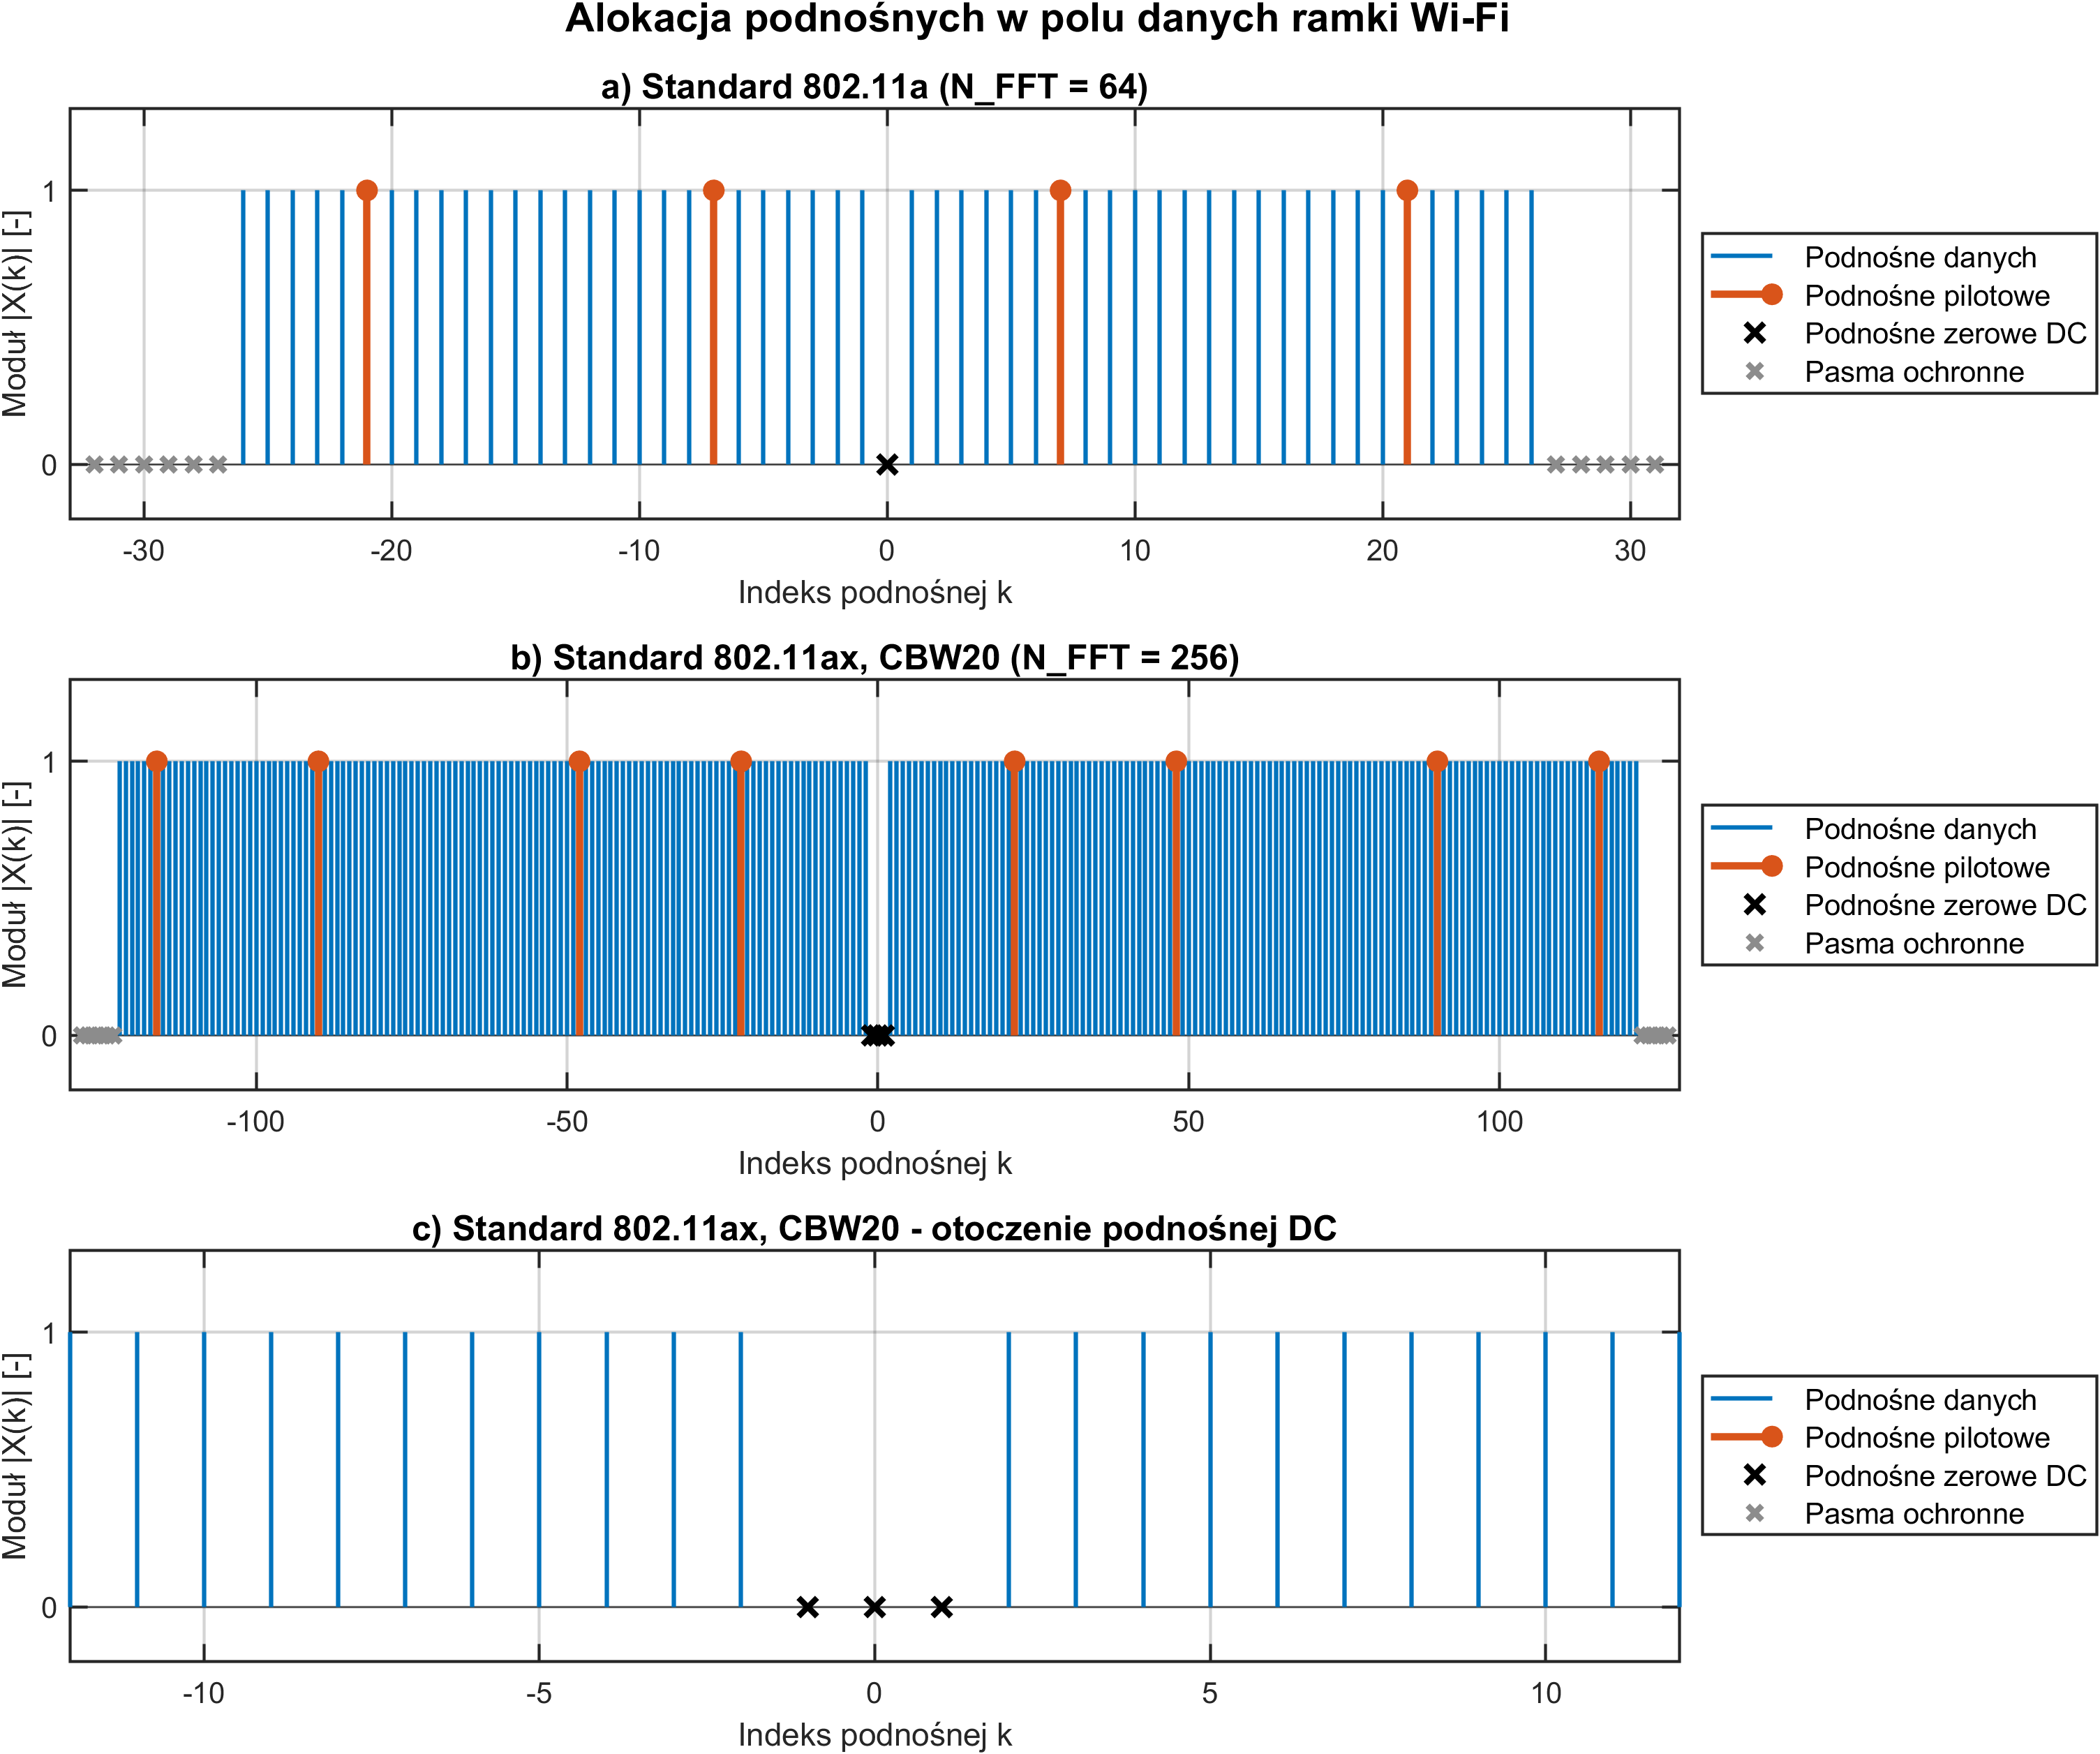
\includegraphics[width=\textwidth]{img/ch2_theory/rys_2_1_alokacja_podnosnych.png}
    \caption{Alokacja podnośnych w~polu danych: a)~802.11a, b)~802.11ax przy szerokości kanału 20~MHz, c)~powiększenie otoczenia podnośnej DC w~802.11ax. Podnośne zerowe zaznaczono krzyżykami na poziomie zera}
    \label{fig:subcarrier_allocation}
\end{figure}

Rozkład podnośnych w~paśmie na przykładzie kanału 20~MHz przedstawiono na rysunku~\ref{fig:subcarrier_allocation}. Podnośne pilotowe służą odbiornikowi komunikacyjnemu do śledzenia fazy i~zajmują ściśle określone pozycje w~siatce częstotliwościowej. Skrajne podnośne pozostawiono puste jako pasma ochronne, ograniczające emisję poza przydzielonym kanałem. Wyzerowano również podnośną centralną $k = 0$, a~w~standardzie 802.11ax grupę od 3 do 23 podnośnych wokół środka pasma (przy czym w~kanale 160~MHz, złożonym z~dwóch podkanałów 80~MHz, oprócz 23 podnośnych centralnych wyzerowane są także po 5 podnośnych w~środku każdego podkanału) \cite{2021}. W~odbiornikach radiowych na zerowej częstotliwości pośredniej naturalnie powstaje silny prążek zakłóceń od napięcia stałego oraz wewnętrznego oscylatora -- brak transmisji na tych podnośnych zapobiega więc zniekształceniu danych.

Alokacja podnośnych przenosi się bezpośrednio na właściwości wyznaczanej mapy odległość--prędkość:
\begin{itemize}
    \item Pasma ochronne ograniczają efektywnie zajęte pasmo (w~kanale 20~MHz do ok.~16,6~MHz w~802.11a oraz 19,1~MHz w~802.11ax), co determinuje rozdzielczość odległościową (podrozdział~\ref{subsec:pbr_fundamentals}).
    \item Wyzerowane podnośne DC tworzą nieciągłość (dziurę) wewnątrz widma, co po transformacji Fouriera podnosi tło listków bocznych w~osi odległości \cite{braun2014}. Zjawisko to kompensuje się za pomocą wielopunktowej interpolacji liniowej brakujących podnośnych na podstawie sąsiednich podnośnych aktywnych (podrozdział~\ref{subsec:clutter_filtering}).
    \item Zmienna amplituda punktów konstelacji QAM w~polu danych powoduje wzmocnienie szumu estymaty kanału przy dzieleniu odebranych podnośnych przez podnośne wzorcowe, co szczegółowo przeanalizowano w~podrozdziale~\ref{subsec:channel_estimation} i~zbadano w~podrozdziale~\ref{subsec:sim_mcs_noise_enhancement}.
    \item Czterokrotnie mniejszy odstęp podnośnych w~802.11ax wydłuża czas trwania symbolu z~4,0 do 13,6~$\mu$s. Zwiększa to zasięg jednoznaczny, lecz proporcjonalnie obniża maksymalną jednoznaczną prędkość radaru (podrozdział~\ref{subsec:pbr_fundamentals}).
\end{itemize}

\subsection{Model matematyczny sygnału OFDM}
\label{subsec:ofdm_modulation}

W~modulacji OFDM strumień danych dzieli się na wiele równoległych podstrumieni i~wysyła jednocześnie na gęsto rozmieszczonych podnośnych. Aby sąsiednie podnośne nie zakłócały się nawzajem, ich odstęp częstotliwościowy musi być odwrotnością czasu trwania części użytecznej symbolu: $\Delta f = 1/T_u$. Ponieważ każdy symbol w~czasie użytecznym jest ograniczony oknem prostokątnym o~długości $T_u$, widmo pojedynczej podnośnej o~częstotliwości środkowej $k\Delta f$ ma kształt przesuniętej funkcji interpolującej $\mathrm{sinc}((f - k\Delta f)T_u)$. Miejsca zerowe tej funkcji przypadają w~odstępach będących wielokrotnościami $1/T_u = \Delta f$, a~więc dokładnie na częstotliwościach środkowych wszystkich pozostałych podnośnych \cite{zielinski2007}. W~rezultacie podnośne pozostają wzajemnie ortogonalne i~nie wnoszą do siebie zakłóceń (ang. \textit{Inter-Carrier Interference}, ICI).

W~nadajniku bity danych są odwzorowywane na zespolone symbole konstelacji $X[k,l]$. Tworzą one dwuwymiarową siatkę, w~której indeks $k$ oznacza numer podnośnej (częstotliwość), natomiast $l \in \{0, 1, \dots, M-1\}$ określa numer kolejnego symbolu OFDM wzdłuż osi czasu wolnego, przy czym $M$ to całkowita liczba symboli w~przetwarzanej ramce (pakiecie). Choć cyfrowe przetwarzanie sygnałów w~radarze operuje na próbkach dyskretnych, propagacja fal radiowych w~otoczeniu zachodzi w~czasie ciągłym. Zjawiska radiolokacyjne -- opóźnienie echa $\tau = 2R/c$ oraz rotacja fazy wywołana prędkością celu $e^{j 2\pi f_D t}$ -- oddziałują na fizyczną falę elektromagnetyczną w~przestrzeni. Z~tego względu opis matematyczny rozpoczyna się od modelu w~czasie ciągłym. Zespoloną obwiednię pojedynczego, $l$-tego symbolu OFDM w~paśmie podstawowym opisuje zależność \cite{braun2014}:
\begin{equation}
    s_l(t) = \frac{1}{\sqrt{N_{\mathrm{FFT}}}} \sum_{k \in \mathcal{K}_{\mathrm{act}}} X[k,l]\, e^{j 2\pi k \Delta f (t - T_{\mathrm{CP}})}, \quad t \in [0, T_{\mathrm{sym}}],
    \label{eq:ofdm_continuous}
\end{equation}
gdzie:
\begin{itemize}
    \item $s_l(t)$ to zespolony sygnał pasma podstawowego $l$-tego symbolu,
    \item $\mathcal{K}_{\mathrm{act}}$ oznacza zbiór indeksów podnośnych aktywnych (przenoszących dane i~piloty, zgodnie z~tabelą~\ref{tab:wifi_params}),
    \item $X[k,l]$ to zespolony symbol konstelacji modulujący $k$-tą podnośną w~$l$-tym symbolu,
    \item $e^{j 2\pi k \Delta f (t - T_{\mathrm{CP}})}$ to zespolona harmoniczna o~częstotliwości $k\Delta f$; przesunięcie o~czas trwania prefiksu $T_{\mathrm{CP}}$ sprawia, że faza fali wynosi zero na początku części użytecznej ($t = T_{\mathrm{CP}}$), natomiast w~przedziale $t \in [0, T_{\mathrm{CP}}]$ funkcja ta okresowo kopiuje końcowy fragment symbolu, tworząc prefiks cykliczny,
    \item $1/\sqrt{N_{\mathrm{FFT}}}$ stanowi współczynnik normalizujący energię sygnału,
    \item $t \in [0, T_{\mathrm{sym}}]$ określa czas trwania pełnego symbolu wraz z~prefiksem cyklicznym ($T_{\mathrm{sym}} = T_u + T_{\mathrm{CP}}$).
\end{itemize}

W~odbiorniku cyfrowym sygnał jest przetwarzany w~postaci próbek pobieranych z~częstotliwością $f_s = N_{\mathrm{FFT}}\Delta f = 1/T_s$. Podstawiając chwile próbkowania części użytecznej $t - T_{\mathrm{CP}} = n T_s = n / (N_{\mathrm{FFT}}\Delta f)$ do równania~\eqref{eq:ofdm_continuous}, czynnik harmoniczny upraszcza się do $e^{j 2\pi k n / N_{\mathrm{FFT}}}$. W~konsekwencji próbki części użytecznej symbolu generuje się bezpośrednio za pomocą $N_{\mathrm{FFT}}$-punktowej odwrotnej dyskretnej transformaty Fouriera (IFFT) \cite{zielinski2007}:
\begin{equation}
    s[n, l] = \frac{1}{\sqrt{N_{\mathrm{FFT}}}} \sum_{k=0}^{N_{\mathrm{FFT}}-1} X[k,l]\, e^{j \frac{2\pi k n}{N_{\mathrm{FFT}}}}, \quad n \in \{0, 1, \dots, N_{\mathrm{FFT}}-1\}.
    \label{eq:ofdm_discrete_ifft}
\end{equation}
Dla podnośnych nieaktywnych (pasm ochronnych oraz zerowych prążków DC, $k \notin \mathcal{K}_{\mathrm{act}}$) przyjmuje się $X[k,l] = 0$.

Przed wysłaniem symbolu w~kanał radiowy na jego początek dołącza się prefiks cykliczny (ang. \textit{Cyclic Prefix}, CP). Jest to powtórzenie końcowych $N_{\mathrm{CP}}$ próbek części użytecznej obliczonej ze wzoru~\eqref{eq:ofdm_discrete_ifft}. Całkowity czas trwania symbolu wynosi wówczas:
\begin{equation}
    T_{\mathrm{sym}} = T_u + T_{\mathrm{CP}} = \frac{N_{\mathrm{FFT}} + N_{\mathrm{CP}}}{f_s}.
    \label{eq:ofdm_symbol_duration}
\end{equation}
W~radarze pasywnym prefiks cykliczny zapewnia dwie fundamentalne korzyści:
\begin{enumerate}
    \item \textbf{Ochrona przed interferencją międzysymbolową (ISI):} dopóki maksymalne opóźnienie echa w~kanale spełnia warunek $\tau_{\max} \le T_{\mathrm{CP}}$, wszystkie opóźnione repliki z~poprzedniego symbolu wygasają wewnątrz bufora $T_{\mathrm{CP}}$. Dla podstawowego czasu $T_{\mathrm{CP}} = 0{,}8~\mu$s odpowiada to maksymalnemu zasięgowi wolnemu od interferencji międzysymbolowej $\Delta R_{\mathrm{CP}} = c T_{\mathrm{CP}} / 2 \approx 120$~m, co z~dużym zapasem pokrywa zasięg wewnątrzbudynkowy \cite{braun2014}. W~standardzie 802.11ax dostępne są także dłuższe prefiksy ($1{,}6$ oraz $3{,}2~\mu$s), zwiększające $\Delta R_{\mathrm{CP}}$ odpowiednio do 240~m i~480~m kosztem dłuższego czasu trwania symbolu $T_{\mathrm{sym}}$.
    \item \textbf{Przekształcenie splotu liniowego w~kołowy:} w~kanale wielodrogowym sygnał nadany ulega splotowi liniowemu z~odpowiedzią impulsową otoczenia. Okresowe powtórzenie próbek w~prefiksie sprawia, że dla części użytecznej symbolu operacja ta staje się splotem kołowym \cite{zielinski2007}. W~odbiorniku po odrzuceniu prefiksu i~wykonaniu transformaty FFT splot kołowy przechodzi w~zwykłe mnożenie punkt po punkcie. Wpływ kanału na każdej podnośnej sprowadza się wówczas do wymnożenia nadanego symbolu $X[k,l]$ przez zespoloną transmitancję $H[k,l]$ \cite{braun2014}.
\end{enumerate}

W~przetwarzaniu radarowym istotną rolę odgrywają również właściwości symboli $X[k,l]$. Sekwencje treningowe preambuły oraz podnośne pilotowe stosują modulację BPSK, w~której każdy punkt ma stałą, jednostkową amplitudę ($|X[k,l]| = 1$). W~polu danych rodzaj modulacji wynika natomiast z~zastosowanego schematu MCS \cite{1999,2021}. Modulacje najniższego rzędu (BPSK, QPSK) zachowują stałą energię symboli ($|X[k,l]|^2 = 1$). Z~kolei modulacje wyższych rzędów (16-QAM, 64-QAM, a~w~802.11ax do 1024-QAM) cechują się nierównomiernym rozkładem energii w~konstelacji. Wewnętrzne punkty takich konstelacji mają energię wielokrotnie niższą od energii średniej ($|X[k,l]|^2 \ll 1$). Gdy odbiornik radarowy dokonuje estymacji odpowiedzi częstotliwościowej kanału przez dzielenie element po elemencie podnośnych odebranych przez podnośne wzorcowe, dzielenie przez tak małe wartości prowadzi do silnego wzmocnienia szumu tła \cite{braun2014,wypich2026}. Mechanizm ten przeanalizowano szczegółowo w~podrozdziale~\ref{subsec:channel_estimation}, natomiast jego wpływ na wykrywalność celów zbadano w~podrozdziale~\ref{subsec:sim_mcs_noise_enhancement}.
